\section{Introduction}
For this project, it is requested to design a mechanical system that can lift a Rzeppa half-shaft constant velocity end joint with a specially designed gripper starting from the base frame of a \texttt{Jodell} gripper. The half-shaft joint is positioned on a tray designed according to its dimensions, from which the gripper will lift the same object.

\subsection{Constant Velocity joint}
A constant-velocity joint (also called a CV joint or homokinetic joint) is a mechanical connection between two rotating shafts, that keeps them rotating at the same speed, while allowing the shafts to be at an angle to each other as they rotate. This joint operates without an appreciable increase in friction or backlash and compensates for the angle between the two shafts, within a certain range of angles.
A common use of CV joints is in front-wheel drive vehicles, where they are used to transfer the engine's power to the front wheels while still allowing the wheels to steer.
A Rzeppa joint consists of a spherical inner shell with 6 grooves in it and a similar enveloping outer shell. Each groove guides one ball. The input shaft fits in the center of a large, steel, star-shaped "gear" that nests inside a circular cage. The cage is spherical but with ends open, and it typically has six openings around the perimeter. 

\subsubsection{Half-shaft end joint}
For this application, we consider a Rzeppa half-shaft constant velocity end joint. Due to its asymmetric structure, its mass is not equally distributed and the center of mass is shifted toward the bulkier head of the joint. Consequently, during lifting, the component tends to tilt under gravity. 

The main design challenge was to determine the optimal grasp location for the modified \texttt{Jodell} gripper while stabilizing the asymmetric load to prevent rotation. Since the joint is made of high-strength metals, structural deformation under clamping force was not a concern. Instead, the design focused on grasping the cylindrical shaft while the part lies horizontally on a custom tray, managing the gravity-induced momentum. Later in this report, we detail how this stabilization was resolved and how the gripper was dimensioned to accommodate a range of automotive shaft diameters.

Its principal measurements are: $90\text{ mm}$ for the head diameter, $23\text{ mm}$ for the threaded section, and $100\text{ mm}$ as the span for stabilization and grasping contacts. Specifically, the grasping claws operate on the intermediate $28\text{ mm}$ diameter (non-threaded) section of the cylinder, whereas the buffer stabilization system acts on the $23\text{ mm}$ diameter threaded section. Images of the physical component and the corresponding 3D CAD model (imported into Creo 9.0.10.0 from SolidWorks) are shown below.

\begin{figure}[H]
    \centering
    \begin{minipage}{0.43\textwidth}
        \centering
        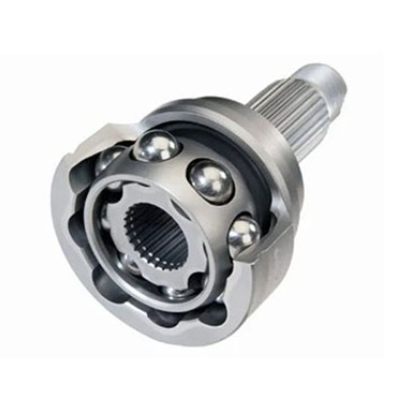
\includegraphics[width=\textwidth]{Immagini/Half-shaft/rzeppa half-shaft.png}
        \caption{Rzeppa's Half-shaft end joint}
    \end{minipage}
    \hfill
    \begin{minipage}{0.43\textwidth}
        \centering
        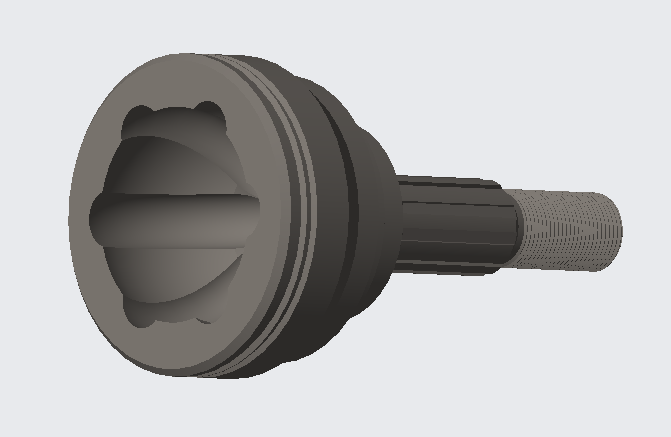
\includegraphics[width=\textwidth]{Immagini/Half-shaft/Half-shaft.png}
        \caption{Half-shaft end joint}
    \end{minipage}
\end{figure}

\begin{figure}[H]
    \centering
    \begin{minipage}{0.35\textwidth}
        \centering
        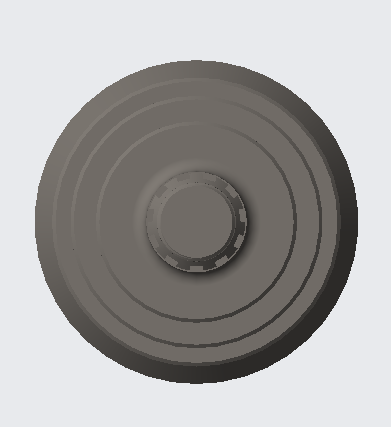
\includegraphics[width=\textwidth]{Immagini/Half-shaft/Half-shaft back .png}
        \caption{Half-shaft end joint back view}
    \end{minipage}
    \hspace{2cm}
    \begin{minipage}{0.35\textwidth}
        \centering
        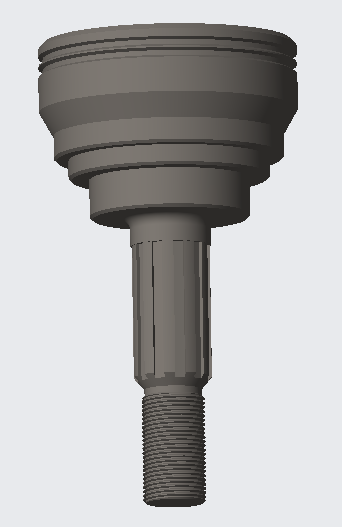
\includegraphics[width=\textwidth]{Immagini/Half-shaft/Half-shaft front.png}
        \caption{Half-shaft end joint upper view}
    \end{minipage}
\end{figure}

\subsection{Design requirements and constraints}
Before detailing the gripper architecture, the geometric and functional constraints dictated by the half-shaft end joint are formally summarized below. These constraints guided every design choice made throughout the development process, including the scrapped attempts discussed in Section~2.

\begin{itemize}
    \item \textbf{Graspable diameter range:} the gripper must accommodate half-shaft sections between $25\text{ mm}$ and $35\text{ mm}$ in diameter, covering approximately $90\%$ of the half-shaft end joints available on the automotive market.
    \item \textbf{No-touch zones:} due to the intricate geometry of the Rzeppa joint (splined input shaft, ball cage, and both threaded sections), most of the component's surface cannot be grasped without risking damage to delicate features. The gripper is therefore restricted to only two contact regions: the intermediate $28\text{ mm}$ non-threaded cylindrical section (claws) and the $23\text{ mm}$ threaded section near the shaft end, which can only be touched axially by the buffer, never radially clamped.
    \item \textbf{Surface protection:} every contact point must be coated with a rubber layer. This is a direct consequence of the no-touch constraint above: since the only accessible surfaces are either toothed or threaded, any rigid metal-on-metal contact would wear down the finish or cause slippage during repeated grasping cycles.
    \item \textbf{Load stability:} because the joint's center of mass is shifted toward the bulkier head, the gripper must counteract the resulting gravity-induced moment to keep the half-shaft horizontal during transport, without relying on structural deformation of the (high-strength metal) component.
    \item \textbf{Compatibility:} the final mechanism must be actuated exclusively through the two linear sliders of the existing \texttt{Jodell} gripper base frame, without introducing additional motors.
\end{itemize}

\subsection{Tray}
The joint is transported in a trail that keeps it horizontal in the same position in which it must be grasped and conserved. Its design facilitates the grasping operation avoiding unnecessary maneuvers.

\subsection{Gripper}
Considering the joint characteristics, the design of the gripper follows two main strategies: 
\begin{itemize}
	\item Ensuring that the part is not damaged during the transport and gripping process: each contact point must have a small rubber layer. In this way, the toothed finishes are not worn out by the repeated grasping process and slips are avoided. Ensuring this will make the robot operate safely.
	\item Compensating the weight forces that, otherwise, would make the joint rotate if picked with the traditional two "fingers": a mechanical buffer is attached on the other side of the contact point of the gripper. This creates a momentum that stabilizes the half-shaft normally affected by gravity forces, not allowing any possible rotations during the transport. In fact, without the buffer part and only using the gripper, the grasp would be unbalanced. 
\end{itemize} 

\subsection{Final design}
The final design consists of an under-actuated mechanical five bar measured to grasp half-shaft end joints with diameters of the grasped section between $25\text{ mm}$ and $35\text{ mm}$, consisting of the $90\%$ of the joints in the automotive market.
Because of this, a simple cylindrical gripper which only performs a rotation about the axis of a single revolute joint (for both sides) is a too simple solution: it would be a cheap and mechanically simple choice, but that would have been the right one only if it were requested to grasp a single type of cylinder, with only one section to care about. To satisfy the task in a robust way, a more complicated quadrilateral-shaped claw was designed by the members of this group.